\documentclass[a4paper]{article}

\setcounter{secnumdepth}{0}

%Metadata
\title{Kuwaiba Open Inventory Administrator's Manual}
\author{Neotropic SAS}
\date{24.03.2017}

%Imports
\usepackage{graphicx}
\usepackage[utf8]{inputenc}
\usepackage{booktabs}
\usepackage[margin=3cm]{geometry}
\usepackage{color}
\usepackage{framed}
\usepackage{verbatimbox}
\usepackage[toc,page]{appendix}
\usepackage{nameref}

%\usepackage{hyperref}

%Modify some defaults
\setlength{\parindent}{0pt} %don't indent new paragraphs

\begin{document}
	\maketitle
	\pagenumbering{gobble}
	
	
	
	\begin{figure}[b]
		\centering System Version \textbf{1.5}
			
		Visit \textbf{kuwaiba.org} for documentation, latest updates and upcoming events
	\end{figure}
	
	
	\newpage
	
	\tableofcontents

	\newpage
	\section{Document History}
		\begin{table}[h!]
			\centering
			\begin{tabular}{l||p{10cm}} %Each letter tells the parser what alignment should have every column
				\toprule
				\textbf{Date} & \textbf{Comments}  \\
				\midrule
				January 19th 2011 & First version. It uses the number 0.3 just to keep compatibility with the version used for the user manual\\
				\midrule
				March 17th 2011 & Corrections regarding to the changes made in the version 0.3 beta 2 \\
				\midrule
				November 8th 2011 & Added details related to the database setup. Added a troubleshooting section \\
				\midrule
				May 22nd 2012 & Adaptation to version 0.4 \\
				\midrule
				July 13th 2012 & Multiple fixes and clarifications \\
				\midrule
				December 12th 2013 & Style corrections \\
				\midrule
				January 19th 2015 & Corrected how the rmiregistry is launched \\
				\midrule
				July 27th 2016 & Adapted to Kuwaiba version 1.0. LaTeX is now used instead of LibreOffice to create the documentation. \\
				\midrule
				December 9th 2016 & Added notes about configuring Glassfish to start on boot. \\
				\midrule
				March 24th 2017 & Added notes about configuring Glassfish to support HTTP compression. \\
				\midrule
				June 1st 2017 & Added Appendix E Configuring Update Center\\
				\bottomrule
			\end{tabular}	
				
		\end{table}
	\newpage
	\section{License}
		\begin{table}[ht]
			\centering
			\begin{tabular}{cp{10cm}}
				
				
\includegraphics[]{img/cc_license_logo.jpg} & This document is published under the terms of a license Creative Commons by-nc-sa. You can find details about it at\linebreak
				\textbf{http://creativecommons.org/licenses/by-nc-sa/2.0/ } \\

				
\includegraphics[width=2cm]{img/osi_logo.jpg} & Kuwaiba Server and Client are licensed under EPL v1 and GPL v2. You can find the whole text of these licenses at \linebreak
				\textbf{http://www.eclipse.org/legal/epl-v10.html} \linebreak
				\textbf{http://www.gnu.org/licenses/old-licenses/gpl-2.0.html} \\
			\end{tabular}
		\end{table}
		\paragraph{Disclaimer} \hspace{0pt}
		\begin{itemize}
			\item Netbeans and Java are registered trademarks of Oracle and/or its affiliates. Other names may be trademarks of their respective owners. The Kuwaiba project is not endorsed by any of them.
			
			\item This document is provided “as is”, with no warranty at all. Install the software and follow the instructions included at your own risk.
			
			\item Kuwaiba uses third-party components with compatible open source licenses (LGPL, BSD-like, etc). You can find a complete list at the project's web page.
		\end{itemize}
	
	\newpage
	\pagenumbering{arabic}
	\section{Introduction}
		Kuwaiba is a plain client/server application. It's Java on both sides, though it's fairly easy to implement clients in any language, since the server exposes a comprehensive SOAP web service interface, which is the native way it talks to the default client and third-party applications. 
		
		In the figure below, you can see a simplified block diagram of the server application.
		\begin{figure}[h!] %h! Means "here" and "!" means override 
			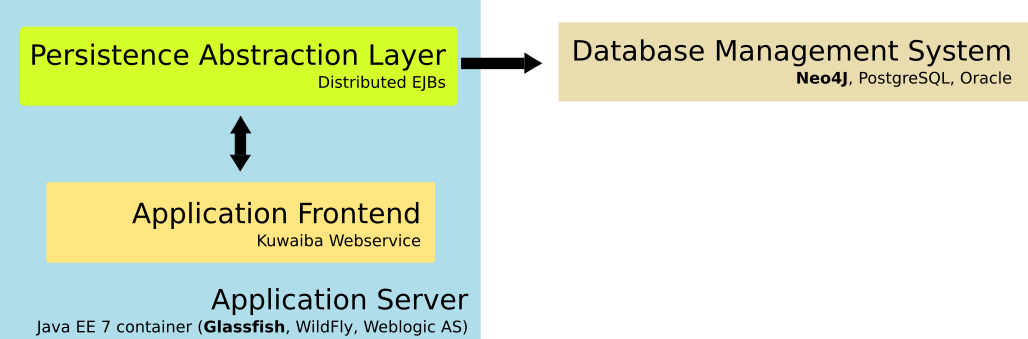
\includegraphics[width=\linewidth]{img/block-diagram.png}
			\caption{Simplified server architecture}
		\end{figure}
		
		We won't go into technical details here, suffice to say that there are three main blocks that are important to keep in mind, as all the troubleshooting procedures will revolve around them. The lower level component is the database. Kuwaiba uses a graph-oriented database called Neo4J. After a few releases using a conventional relational database, we realized that the best way to model a telecommunications network is not a set of related tables, but a graph. Neo4J may work in two modes: as a server responding JSON requests on a TCP port or as an embedded database, when the application access the database files directly without any service mediating between the application and the data. Kuwaiba uses the latter. This means that you can't access the database while Kuwaiba is running, because it will be locked. Running Neo4J in embedded mode increases the performance, sacrificing accessibility to the data.\newline
		
		The middle layer is called the Persistence Service. This is one of the most important components, and it's responsible for accessing the information stored in the database in a safe way, isolating that logic from the rest of the application. Other layers of the application will never know that the backend is Neo4J thanks to this module, and this enables the development of implementations using other DBMS like Oracle, for example. It's called a service for historic reasons: Prior to version 1.0 this component was a standalone application that ran in a different JVM than the one used by the application server. This was complicated to setup, so it was merged with the application running on the application server. However, It still runs when the application is deployed or at application server (AS) startup. You should check the AS log files to see if the Persistence Service is running correctly, or nothing else will work.\newline
		
		The third component is the frontend of the server. It implements the web service that allows the communication between the server and its clients or third party applications. In a general sense, it's a northbound interface. As we will see later, you will be able to access a simple web-based interface to perform administrative tasks, like resetting passwords or creating the default database structure. Also, you will be able to access the WSDL that would eventually allow you to integrate in-house applications.\newline
		
		As you can see, this is pretty straightforward and once it's done the first time, it can easily be reproduced. Starting from scratch, given that all requirements are already downloaded, the server can be configured and started in less than 10 minutes.
	\newpage
	
	\section{Server Installation}
		The server application can be installed on any platform supported by Java EE in all its implementations (OpenJDK, Oracle's JDK, etc). The instructions are basically the same for all platforms, and the differences will be highlighted when necessary.
		\subsection{Requirements}
			\begin{itemize}
				\item JDK 7 or superior. On Windows platforms, you'll need to download it from the Oracle's website\footnote{Oracle's JDK Downloads http://www.oracle.com/technetwork/java/javase/downloads/index.html}, while on Linux or BSDs systems you can use the package/port managers to install OpenJDK from a repository. Refer to the documentation of your distribution for more details on how to install Java.
				\begin{framed} {\large \textbf{Important}} \\
					Note that you need the JDK (Java Development Kit), not only the JRE (Java Runtime Environment).
				\end{framed}
				\item An application server. The instructions presented in this document apply to Glassfish version 3 or above, however, Glassfish 4.1 is highly recommended. You can find details on its installation process here\footnote{Glassfish Quick Start Guide https://glassfish.java.net/docs/4.0/quick-start-guide.pdf}. In short, just download the .exe/.bin installer from its official site\footnote{Glassfish Official Web Site https://glassfish.java.net/} and execute it choosing the default options. Make sure you secure and tune it in your production environment. You can also use any other Java EE 7 compliant application server, but this document will use Glassfish.
				\item Neo4J 2.3.x Community Edition. We just need some libraries included in its installation package, but it's good to have it all installed so we can use it for troubleshooting problems in the future. You can get the installer from here\footnote {Neo4J 2.3.2 Community Edition Downloads https://neo4j.com/download-thanks/?edition=community\&flavour=unix\&release=2.3.2}.
				\begin{framed} {\large \textbf{Important}} \\
					Neo4J libraries are no longer distributed in the server installation package due to open source licenses conflicts.
				\end{framed}
				\item The latest Kuwaiba Server installation package. You can get it from here\footnote {Kuwaiba Installation Packages http://sourceforge.net/projects/kuwaiba/files/}. As of version 1.0, both client and server are in the same file, whose name must look like this 
		
				\begin{verbatim}
					kuwaiba\_[version]\_[alpha/beta/stable].zip
				\end{verbatim}
				
			\end{itemize}
		
		
		\newpage
		\subsection{Step by Step Guide}
		\subsubsection{Step 1: Preparation}
			Let's take a look at the structure of the server installation package:
			
			\begin{table}[h!]
				\begin{tabular}{p{5cm}p{10cm}}
					\toprule
					dbs & 
					In this directory you will find default databases you can use to get started with Kuwaiba.
					\begin{itemize}
						\item \textbf{01\_empty\_kuwaiba.db.zip}: Contains the database schema plus a default user account.
						\item \textbf{02\_containment\_kuwaiba.db.zip}: Contains the database schema, a default user account and a sample containment hierarchy but no objects.
						\item \textbf{03\_data\_kuwaiba.db.zip}: Contains the same as 02\_containment\_kuwaiba.db plus some objects, views and tasks 
						
					\end{itemize} \\
					\midrule
					updates.zip & This file contains a updates.xml file and the set of Netbeans module file (.NBM) for the current Kuwaiba version. See \textbf{\nameref{app:AppendixE}}\\
					\midrule
					KuwaibaServer.ear & The enterprise application to be deployed on the application server \\
					\midrule
					README & A simple README file with useful information about where to get resources. \\
					\midrule
					THIRDPARTY & The list of open source, third-party components used in the server, as well of their respective licenses and links to the original projects. \\
					\midrule
					LICENSE.EPL & Text of the EPLv1 license \\
					\midrule
					LICENSE.GPLv2 & Text of the GPLv2 license \\
					\midrule
					CHANGELOG & List of changes since the first version \\
					\midrule
					class\_hierarchy.xml & A default database schema that can be uploaded instead of using one of the default databases. Only for experimented users. \\
					\bottomrule	
				\end{tabular}
			\end{table}
			Before proceeding with the formal installation we must configure some things:
			\begin{itemize}
				\item Create the directory where the database will be stored. Make sure the user that will run Glassfish has read and write permissions on that directory. If you want to create the database from scratch, leave this directory empty, otherwise, unzip one of the default databases and copy it there (recommended). The default database location is \textbf{/data/db/kuwaiba.db}
				\item Create a directory to store the backgrounds and other files. Also make sure the user that will run Glassfish has read and write permissions on that directory. The default backgrounds folder location is \textbf{/data/img/backgrounds}.
				\item If you are going to use the default locations (/data/db/kuwaiba.db and /data/backgrounds), skip this step, otherwise, open the file \textbf{KuwaibaServer.ear} and search for the file  \textbf{KuwaibaServer-ejb.jar/META-INF/ejb-jar.xml}. Note that both \textbf{KuwaibaServer.ear} and \textbf{KuwaibaServer-ejb.jar} are simply .zip files with other extensions, so you should be able to open them with any zip manipulation utility. Modern programs allow you to modify the files contained within zip files and they will update the original compressed file.\\ 
				
				\textbf{ejb-jar.xml} is an XML file that contains a set of configuration parameters:
				
				\newpage
				\begin{table}[h!]
					\begin{tabular}[h!]{p{5cm}p{10cm}}
						\toprule
						\textbf{Parameter} & \textbf{Description} \\
						\midrule
						dbUsername & Not used \\
						\midrule
						dbPassword & Not used \\
						\midrule
						dbPath & The path where the database is located. \newline \textbf{Default value:} /data/db/kuwaiba.db \\ 
						\midrule
						dbHost & Not used \\
						\midrule
						dbPort & Not used \\
						\midrule
						backgroundsPath & The path where the backgrounds and other files are stored. \newline \textbf{Default value:} /data/img/backgrounds \\
						\midrule
						corporateLogo & The URL of the logo that will be displayed in the reports.  \newline \textbf{Default value:} http://neotropic.co/img/logo\_small.png\\
						\midrule
						enableSecurityManager & Enables the JVM security manager. This could be used to restrict the kind of code that can be executed. See \textbf{\nameref{app:AppendixA}} for details.  \newline \textbf{Default value:} false\\
						\bottomrule
					\end{tabular}
				\end{table}
				
				Set the paths to appropriate values and compress the .ear and jar files if your archiving utility doesn't do it automatically. \textbf{Note:} You can also leave the default values, skip this step, and then modify the file once the whole bundle has been deployed on the application server. It will most likely be in the path:
				\begin{verbbox}
					[GLASSFISH_DIR]/glassfish/domains/domain1/[INSTALLER_FILE_NAME]
				\end{verbbox}
				\begin{figure}[ht]
					\centering	
					\theverbbox
				\end{figure}
				\begin{framed} {\large \textbf{Important}} \\
					If the database directory does not exist or can not be written, the \textbf{Persistence Service won't start}. Check the \textbf{\nameref{sec:Troubleshooting}} section for more details if this happens.
				\end{framed}
				\item Finally, copy all .jar files in the directory \textbf{lib} of the Neo4J's install package to the path
				\begin{verbbox}
					[GLASSFISH_DIR]/glassfish/domains/domain1/lib
				\end{verbbox}
				\begin{figure}[ht]
					\centering	
					\theverbbox
				\end{figure}				
			\end{itemize}
			\subsubsection{Step 2: Deploying the application}
			\begin{itemize}
				\item Open a command prompt/console and start Glassfish by typing this:
				\begin{verbbox}
					[GLASSFISH_DIR]/bin/asadmin start-domain domain1
				\end{verbbox}
				\begin{figure}[h!]
					\centering	
					\theverbbox
				\end{figure}
				\item Once the application server is up and running, it will provide a web management interface listening on port 4848 (http://[server\_domain\_name\_or\_ip]:4848). Don't forget the credentials you provided during the server installation process because they will be used for further administration procedures. See figure~\ref{fig:gf_mgmconsole}.
				\begin{figure}[h!]
					\centering
					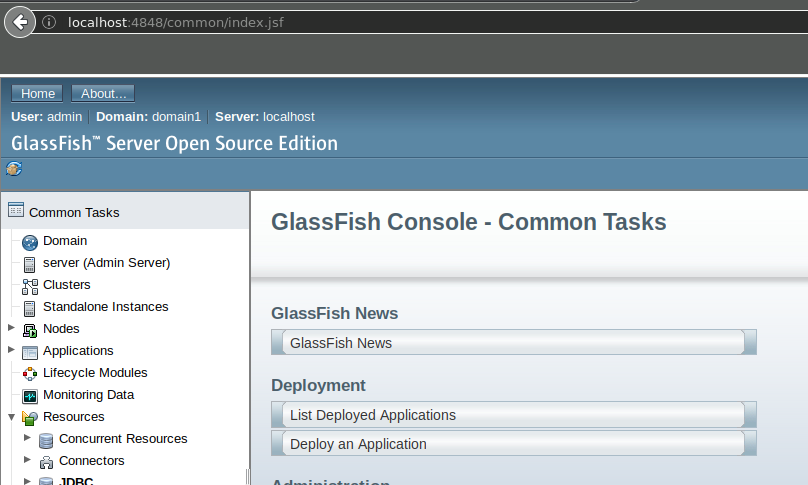
\includegraphics[width=0.8\linewidth]{img/gf_management_console.jpg} 
					\caption{Glassfish management console}
					\label{fig:gf_mgmconsole}
				\end{figure}		
				\item Now you are ready to deploy the enterprise application. Take the EAR file you will find in the server bundle called \textbf{KuwaibaServer.ear} and upload/publish it using the section Applications/Deploy. See figure~\ref{fig:dapplications}.
				\begin{figure}[h!]
					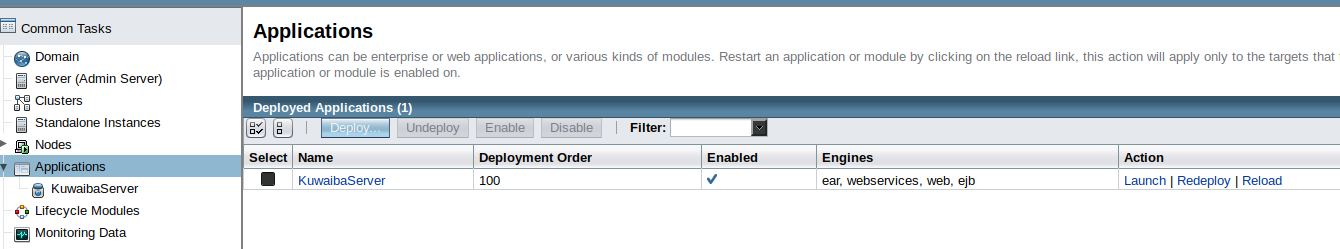
\includegraphics[width=\linewidth]{img/gf_deployed_applications.jpg} 		
					\caption{Deployed applications}
					\label{fig:dapplications}		  
				\end{figure}				
				\item Test if the application was correctly deployed by opening the URL \\ \textbf{http://[server\_domain\_name\_or\_ip]:8080/kuwaiba/}. See figure~\ref{fig:kw_managementconsole}.
				\begin{figure}[h!]
					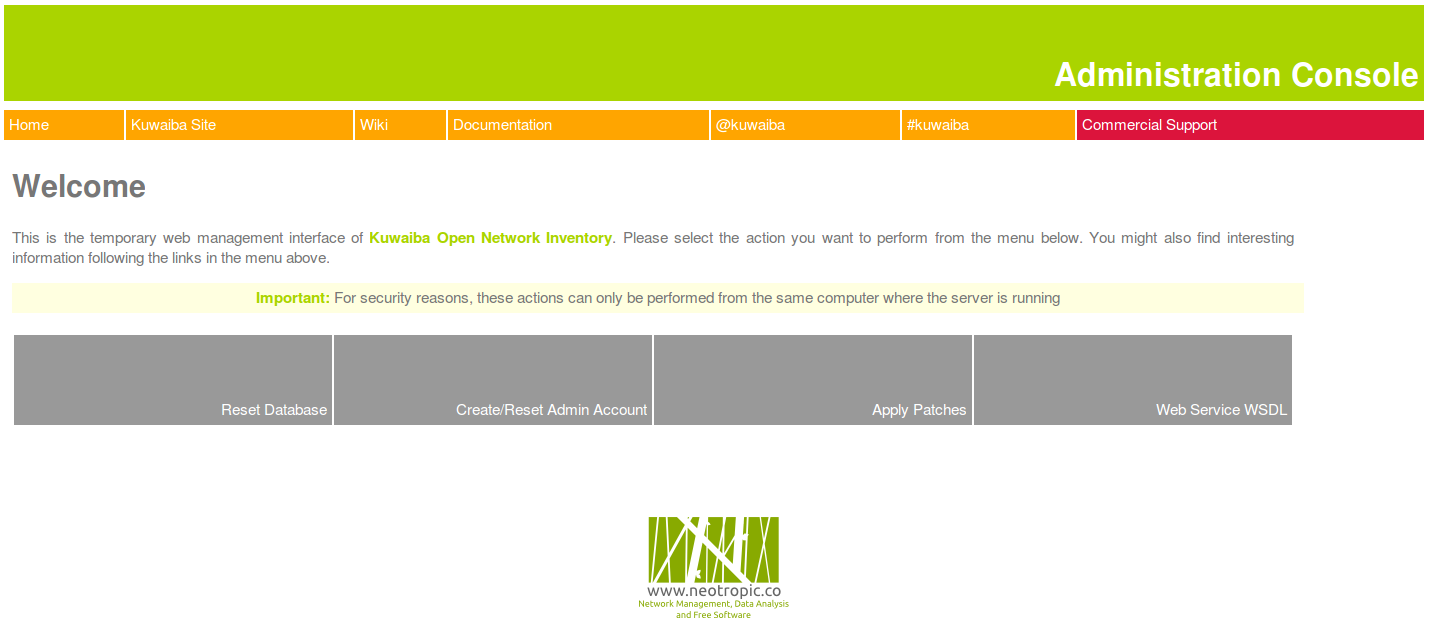
\includegraphics[width=\linewidth]{img/kw_management_console.png} 	
					\caption{Administration console}
					\label{fig:kw_managementconsole}
				\end{figure}
				
				\begin{framed} {\large \textbf{Important}} \\
					For security reasons, the administration console can \textbf{only} be opened from the same computer the server is running. If you try to open it from some other computer, you'll get an error. If you want to access the administration console from outside, you can use an SSH tunnel.
				\end{framed}
				\item Additionally, \textbf{always} check the command prompt/console you used to launch the server to see if an error was thrown. Sometimes, the errors are logged only in the server log file, located at \textbf{[GF\_INSTALL\_DIR]/glassfish/domains/domainXX/logs/}. The application may have been deployed, but the Persistence Service might have not started. A successful startup should look like this in the server log files:
				\begin{figure}[h!]
					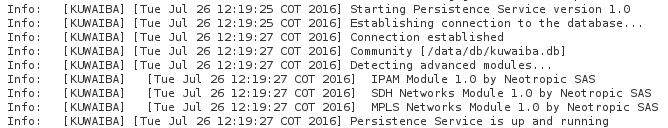
\includegraphics[width=\linewidth]{img/log_messages.png} 	
					\caption{Startup messages}
					\label{fig:startup_messages}
				\end{figure}
			\end{itemize}
			
			\newpage
			\section{Server Side Troubleshooting} \label{sec:Troubleshooting}
				\begin{enumerate}
					\item If you get a \textit{Cant't reach backend} error, it means that the Persistence Service didn't start. The most probable cause is that the database path was not set correctly, or the service does not have written access to it. Check Glassfish log files and search for the "[KUWAIBA]" tag to see the service startup messages. The log file is typically located at:
					\begin{verbbox}
						[GF_INSTALL_DIR]/glassfish/domains/domain1/logs/server.log
					\end{verbbox}
					\begin{figure}[h!]
						\centering	
						\theverbbox
					\end{figure}					
					\item A message \textit{Can not find the class InventoryObject} means that 
					\item If you install Glassfish under MS Windows 7/Vista in \textbf{c:/glassfishv3}, check if you have proper permissions to write on this location, since due to system restrictions it's not possible by default. That will affect the domain creation and application deployment processes.
					\item In some cases, if you install Glassfish before installing the JDK under MS Windows (especially versions 7 and Vista) or when the installer detects a wrong version of Java, the variable AS\_JAVA in \textbf{[GLASSFISH\_INSTALL\_DIR]/glassfish/config/asenv.bat} is set to a wrong location. It should be pointing to the JAVA\_HOME value (this is, the JDK installation directory).
				\end{enumerate}
			\newpage
			\section{Client Installation}
				The client should work on all JRE supported platforms.
				\subsection{Requirements}
					\begin{itemize}
						\item JRE 7 or superior
					\end{itemize}
			
				\subsection{Step by step guide}
					\begin{enumerate}
						\item Download the last stable client bundle. As explained in the past chapter, as of version 1.0, the client and server are included in the same .zip file.
						\item Extract the client files.
						\item Execute the binary suitable for your platform located at
						\begin{verbbox}
							[EXTRACTION_DIR]/kuwaibainventory/bin
						\end{verbbox}
						\begin{figure}[ht]
							\centering	
							\theverbbox
						\end{figure}
						The file is called \textbf{kuwaibainventory.exe} for Windows platforms and \textbf{kuwaibainventory} for Unix-like systems. \textbf{[EXTRACTION\_DIR]} is the directory from where you extracted the files.
						\item You may need to change the file permissions to make the binary executable under Unix-like OS using the command
						\begin{verbbox}
							chmod 755 [EXTRACTION_DIR]/kuwaibainventory/bin/kuwaibainventory
						\end{verbbox}
						\begin{figure}[ht]
							\centering	
							\theverbbox
						\end{figure}	
						
					\end{enumerate}
				\subsection{Client Side Troubleshooting}
				\begin{enumerate}
					\item You are getting an \textit{Unexpected end of file from server} error at login time. You are trying to use HTTP connect to an HTTPS port. Check the connection settings and select "HTTPS".
				\end{enumerate}
		\newpage
		\begin{appendices}
			\appendix
			\section{Appendix A. Security Manager Configuration} \label{app:AppendixA}
			If you have set the \textbf{enableSecurityManager} configuration variable to \textbf{true},create a text file called \textbf{.java.policy} (note the dot before the name). Place it in your user directory (/home/[username] in UNIX environments, or \textbf{c:/Documents and Settings/[username]} or \textbf{c:/users/[username]} in Windows systems). It should contain these lines:
			
			\begin{verbbox}
				grant {
					permission java.util.PropertyPermission "*","read,write";
					permission java.util.PropertyPermission "sun.arch.data.model","read";
					permission java.io.FilePermission "persistence.properties","read";
					permission java.lang.RuntimePermission "accessDeclaredMembers", "read";
					permission java.lang.RuntimePermission "shutdownHooks", "write";
					permission java.lang.RuntimePermission "modifyThread";
					permission java.lang.reflect.ReflectPermission "suppressAccessChecks";
					permission java.net.SocketPermission "127.0.0.1","connect,accept,resolve";
					permission java.io.FilePermission "<<ALL FILES>>","read,write,delete";
				};
			\end{verbbox}
			\begin{figure}[ht]
				\centering	
				\theverbbox
			\end{figure}
			Note that you should NOT run Glassfish as root. These settings can be used if the persistence service AND the application run in the same box (the last line governs who can get connected to the service - in this case, only those applications running in the same computer). You might add some more permissions depending on what other Java applications you are running on that computer. Also, the last two lines can be tuned to be less permissive, if preferred. For more information about permissions, please check the official documentation by Oracle\footnote{Policy files http://docs.oracle.com/javase/1.3/docs/guide/security/PolicyFiles.html} \footnote{Permissions http://docs.oracle.com/javase/6/docs/technotes/guides/security/permissions.html}.
			
			There's also some information on how to apply the security manager rules only to Glassfish here\footnote{The server.policy file https://docs.oracle.com/cd/E18930\_01/html/821-2418/beabx.html}
			
			\newpage
			\appendix
			\section{Appendix B. How to Configure a Secure Connection} \label{app:AppendixB}
				\subsection{Importing a Digital Certificate}
				\textbf{Note:} You can find detailed information about how to manage digital certificates in Glassfish in the Oracle's Java EE documentation \footnote{Working with Digital Certificates https://docs.oracle.com/javaee/6/tutorial/doc/bnbyb.html}. \\
				
				\begin{enumerate}
					\item If you already own a certificate issued by a Certification Authority, skip this step. Otherwise, it means you will use a self-signed certificate. The first time you run Glassfish and/or create a domain, a certificate is generated; you can use that one or generate another with your own corporate information. To do this, execute the following command (the command is located in the \textit{bin} directory of you JDK installation):\\
					
					\small keytool -genkey -keyalg RSA -alias [alias] -keystore [keystore\_filename] -validity 3600 -keysize 2048\\
					
					Where \textit{alias} is the certificate alias (use \textbf{s1as} to match the default settings) and \textit{keystore\_filename} is the name of the file where the certificate keys will be stored (the default name is \textbf{keystore.jks}). Read the command documentation for more information about the other options. Note that this certificate could also be created using other third-party tools, like the \textbf{openssl} command. Take into account that the field \textbf{CN} (the answer to the question \textit{What is your first and last name?}) must match the name of your server. Also, the default password used by Glassfish for the keystore is \textbf{changeit}. If you are OK with the default configuration, use that one, if not, you will have to edit the file [gf-installation]/glassfish/domains/domain1/config/domain.xml file.
					\begin{figure}[h!]
						\centering
						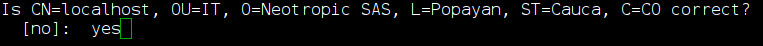
\includegraphics[width=0.7\linewidth]{img/certificate_generation.png} 	
						\caption{Certificate generation}
						\label{fig:certificate_generation}
					\end{figure}
					
					\item If you plan to use more than one certificate in your server or if your certificate was issued by a CA, you need to import it into a keystore that Glassfish can read, otherwise, you can skip this step.  To do that, execute the following command: \\
					
					keytool -import -alias [alias] -keystore [keystore\_filename] -file [CERTIFICATE\_FILE\_NAME]\\
					
					Same recommendations from the past step apply here.
					\item Backup and replace the default keystore in Glassfish [gf-installation]/glassfish/domains/domain1/config/keystore.jks and copy the file created in step 1 (or 2 if you have a certificate issued by a CA). Don't forget to rename the file you generated to \textbf{keystore.jks}. If you use a custom name, you will have to change it as well in the \textbf{domains.xml} file.
					\item Restart the server, open a browser window and go to the URL \textbf{https://[your\_server]:8181/kuwaiba}. You will get a self-signed certificate error. If you open the certificate details, you should see fields you filled in previously. Add this certificate as an exception.
					\newpage
					\begin{figure}[h!]
						\centering
						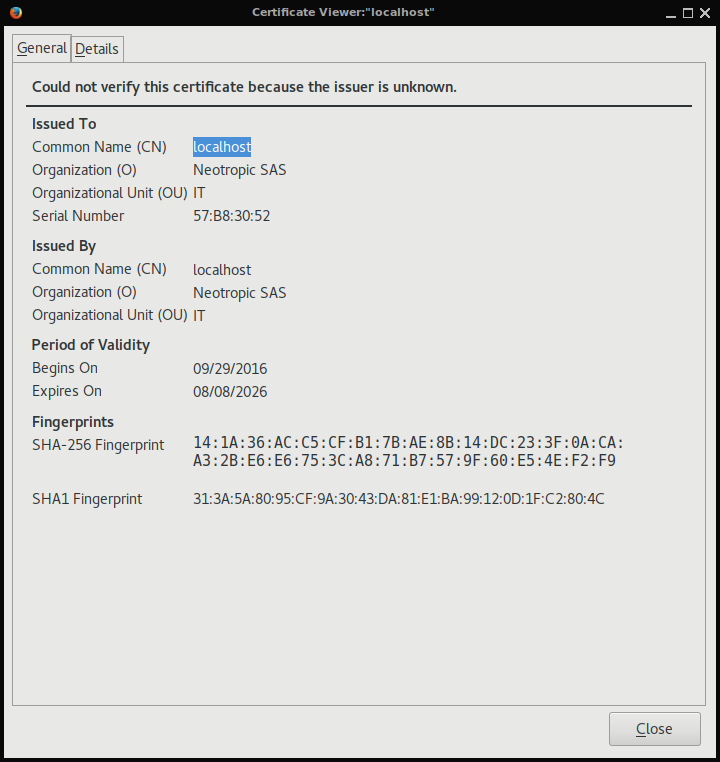
\includegraphics[width=0.7\linewidth]{img/certificate_info.png} 	
						\caption{Self-signed certificate}
						\label{fig:self-signed-certificate}
					\end{figure}
				\end{enumerate}				
				\newpage
				\subsection{Configuring the Client}
				
				If you are using a certificate issued by a CA, the client does not need any additional configuration (don't forget to use the port \textbf{8181} in your connection settings. This port can also be configured using the \textbf{domain.xml} file). If it's a self-signed certificate, you need to tell the client application that the certificate can be trusted (just like you did manually when you added the exception in the web browser). To do this, follow these steps:
				\begin{enumerate}
					\item In the certificate window you opened in the last step there is a \textit{details} tab. The location differs depending on the browser, but it's always there. This example shows the Firefox way:
					
					\begin{figure}[h!]
						\centering
						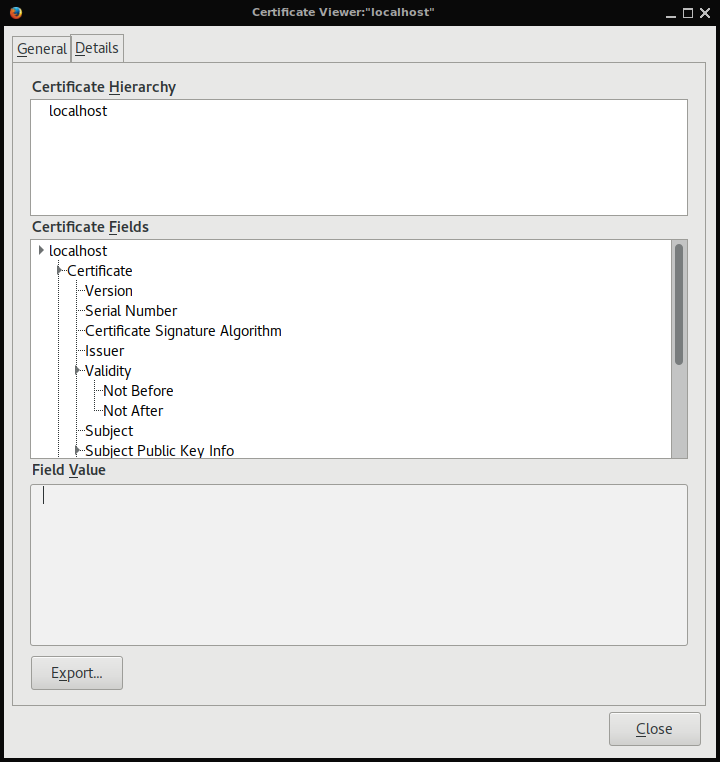
\includegraphics[width=0.6\linewidth]{img/certificate_details.png} 	
						\caption{Certificate details}
						\label{fig:certificate-details}
					\end{figure}
					
					Click on \textit{Export} and export it in a DER format
					\item Using again the \textbf{keytool} command, import it\\
					
					keytool -import -alias [alias] -keystore kuwaiba\_keystore.jks -file [DER\_CERTIFICATE\_FILE\_NAME]\\
					
					Make sure to use as keystore name \textbf{kuwaiba\_keystore.jks}. Copy the resulting file in the directory \textbf{etc} of your client installation.\\
					
					\begin{figure}[h!]
						\centering
						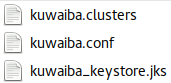
\includegraphics[width=0.2\linewidth]{img/etc_contents.png} 	
						\caption{Contents of \textbf{etc} directory}
						\label{fig:etc-contents}
					\end{figure}
					In the file \textbf{kuwaiba.conf} you can configure the name of the keystore file. The same file can be used for as many clients as you need.
				\end{enumerate}
			\section{Appendix C. Starting Glassfish on Boot} \label{app:AppendixC}
				\subsection{Systemd}
				\begin{enumerate}
					\item Create a file called \textbf{glassfishd.service} in \textit{/etc/systemd/system/} (This location may vary from distribution to distribution) with the following contents:
					\begin{verbbox}
						[Unit]
						Description=Glassfish Server
						
						[Service]
						Type=forking
						
						# Change the user and Glassfish location as needed
						User=kuwaiba
						ExecStart=/home/kuwaiba/apps/glassfish4/bin/asadmin start-domain > /dev/null
						ExecStop=/home/kuwaiba/apps/glassfish4/bin/asadmin stop-domain > /dev/null
						ExecReload=/home/kuwaiba/apps/glassfish4/bin/asadmin restart-domain > /dev/null
						
						# Timeout for the server to start up/shut down process (in seconds)
						TimeoutSec=300
					\end{verbbox}
					\begin{figure}[ht]
						\centering	
						\theverbbox
					\end{figure}\\
					The \textbf{user} means the user that will launch the process. \textbf{ExecStart} is the command used to start the server. \textbf{ExecStop} is the command to stop the server and \textbf{ExecReload} is used to restart the server process. \textbf{TimeoutSec} configures the time to wait for start-up and stop the server process. If the server is stopped right after starting without apparent reason, increase its value.
					\item Enable or disable the service by running as root: 
					\begin{verbbox}
						systemctl enable|disable glassfishd
					\end{verbbox}
					\begin{figure}[ht]
						\centering	
						\theverbbox
					\end{figure}
					\item You can start, stop or check the status of the service by executing the command
					\begin{verbbox}
						systemctl start|stop|status glassfishd
					\end{verbbox}
					\begin{figure}[ht]
						\centering	
						\theverbbox
					\end{figure}\\
					The latter is particularly useful to troubleshoot potential problems.
				\end{enumerate}
				
				\newpage
				\subsection{SysV Init}
				\begin{enumerate}
					\item Create a file called \textbf{glassfishd} in \textit{/etc/init.d} with the following contents:
					\begin{verbbox}
						#!/bin/sh
						
						#
						# Glassfish init script for Linux
						#
						
						#Change the location as needed
						GLASSFISH_HOME=${GLASSFISH_HOME:-"/home/kuwaiba/apps/glassfish4"}
						
						case "$1" in
						start)
						$GLASSFISH_HOME/bin/asadmin start-domain > /dev/null
						;;
						stop)
						$GLASSFISH_HOME/bin/asadmin stop-domain > /dev/null
						;;
						restart)
						$GLASSFISH_HOME/bin/asadmin restart-domain > /dev/null
						;;
						\*)
						echo "Usage: $0 (start|stop|restart|help)"
						esac
					\end{verbbox}
					\begin{figure}[ht]
						\centering	
						\theverbbox
					\end{figure}\\
					Don't forget to change the GlassFish path as needed.
					\item Run this command as root:
					\begin{verbbox}
						update-rc.d glassfishd defaults
					\end{verbbox}
					\begin{figure}[ht]
						\centering	
						\theverbbox
					\end{figure}\\
					\item You can start, stop or restart the server at any moment using the command:
					\begin{verbbox}
						/etc/init.d/glassfish start|stop|restart
					\end{verbbox}
					\begin{figure}[ht]
						\centering	
						\theverbbox
					\end{figure}
					
				\end{enumerate}
			\newpage
			\section{Appendix D. Configuring HTTP Compression on Glassfish} \label{app:AppendixD}
				Since version 1.2, the Kuwaiba client supports HTTP compression. If you experience delays opening views or expanding trees, enable this option on Glassfish and the information exchanged between the clients and the server will be compressed using gzip.
				\begin{enumerate}
					\item Open the Glassfish administration console (http://[SERVER\_IP]:4848) and go to Configurations $\rightarrow$ server-config $\rightarrow$ Network Config $\rightarrow$ Network Listeners.\\
					\begin{figure}[h!]
						\centering
						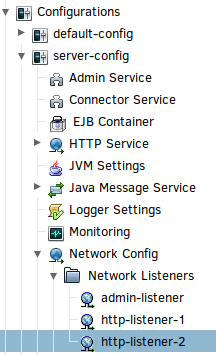
\includegraphics[width=0.2\linewidth]{img/gf_configurations_server_config.png} 	
						\caption{HTTP listeners configuration}
						\label{fig:listeners-config}
					\end{figure}
					\item By default, Glassfish starts three listeners\footnote{Administering HTTP Listeners https://docs.oracle.com/cd/E18930\_01/html/821-2416/ggnfu.html}. You need to modify http-listener-1 (http) and http-listener-2 (https) only. For each one, select the "HTTP" tab.
					\begin{figure}[h!]
						\centering
						
\includegraphics[width=0.4\linewidth]{img/gf_edit_http_listener.png} 	
						\caption{HTTP tab}
						\label{fig:http-tab}
					\end{figure}
					\item Enable compression, make sure "text/xml" is included in the list of compressible MIME types and set the value, in bytes, over which the content is going to be compressed. 2048 is a good default number, but you should change it depending on the size of your views.
					\begin{figure}[h!]
						\centering
						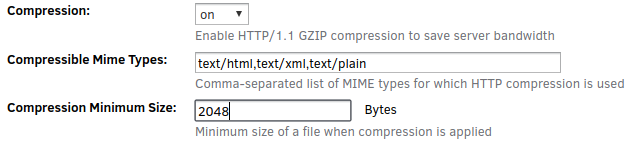
\includegraphics[width=0.7\linewidth]{img/gf_enable_compression.png} 	
						\caption{Enabling compression}
						\label{fig:enabling-compression}
					\end{figure}
				\end{enumerate}
			\newpage
			\section{Appendix E. Configuring Update Center} \label{app:AppendixE}
			Since version 1.5, the Kuwaiba client can be updated using an update center. An \textbf{Update Center} is a set of files which are put in a server to be download by client application. The server can be anyone; e.g., GlassFish, Apache, Apache Tomcat. Once the server is selected, unzip the updates.zip, locate the files in the server and find the URL for the \textbf{updates.xml} file; this URL is used to configure the Kuwaiba client to get the latest version \textbf{figure~\ref{fig:update_center_options}}.
			
			\begin{figure}[h!]
				\centering
				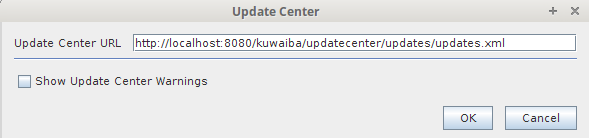
\includegraphics[width=0.7\linewidth]{img/update_center.png}
				\caption{Update Center options}
				\label{fig:update_center_options}
			\end{figure}
						
			 You must configure the update center in the Kuwaiba client. Open the Update Center module look in the menu for Tools $\rightarrow$ Update Center. Once the Update Center URL was assigned, the update must begin right away. For the next Kuwaiba run, if there are updates, the update will be automatical, and if it is necessary to restart the application, it will show a notification to restart.
			\newline
			\newline
			You can decide not to configure a server for the update center. In this case, there is the option to hide the warnings generated in the Kuwaiba client when the update is not found update.xml resource  \textbf{figure~\ref{fig:update_center_options}}.					
			
		\end{appendices}			
\end{document}
